\chapter{User Guide}

The user guide is a tutorial for non-technical users to learn how to use the tool. The tool has been extensively tested on Linux, the tool has full functionality on Linux and basic functionality on Windows.

\section{Installation}

The tool has the following required dependencies:

\begin{itemize}
	\item Python 3
	\item Tkinter
	\item NumPy
	\item Matplotlib
	\item Pillow
\end{itemize}

Tkinter is the default GUI package for Python and Matplotlib depends on NumPy so Tkinter and Matplotlib do not need to be installed explicitly. The tool has the following optional dependencies:

\begin{itemize}
	\item Pyomo
	\item An optimiser, either CPLEX or GLPK
\end{itemize}

The optional dependencies are used to optimise schedules, these are not strictly required as users can input their own schedules. GLPK is recommended because of its licence and open-source development. The source code is found at \texttt{gitlab.doc.ic.ac.uk/mtl115/aes}. Please refer to the package's websites for troubleshooting. Alternatively, contact the author for assistance.

\subsection{Linux Installation}

The tool was tested on Ubuntu 18.04.1. Python is pre-installed so the following packages can be installed as below:
\begin{verbatim}
apt install python3-pip
apt install python-glpk
apt install glpk-utils
pip3 install matplotlib
pip3 install pillow
pip3 install pyomo
\end{verbatim}

\subsection{Windows Installation}

The tool was tested on Windows 10. First, download Python from the official website, then setup the path environment variable so \texttt{python} can be executed on the command prompt. Afterwards, install the basic dependencies as below: 

\begin{verbatim}
python -m pip install matplotlib
python -m pip install pillow
python -m pip install pyomo
\end{verbatim}

\section{Usage}

\begin{figure}[H]
	\centering
	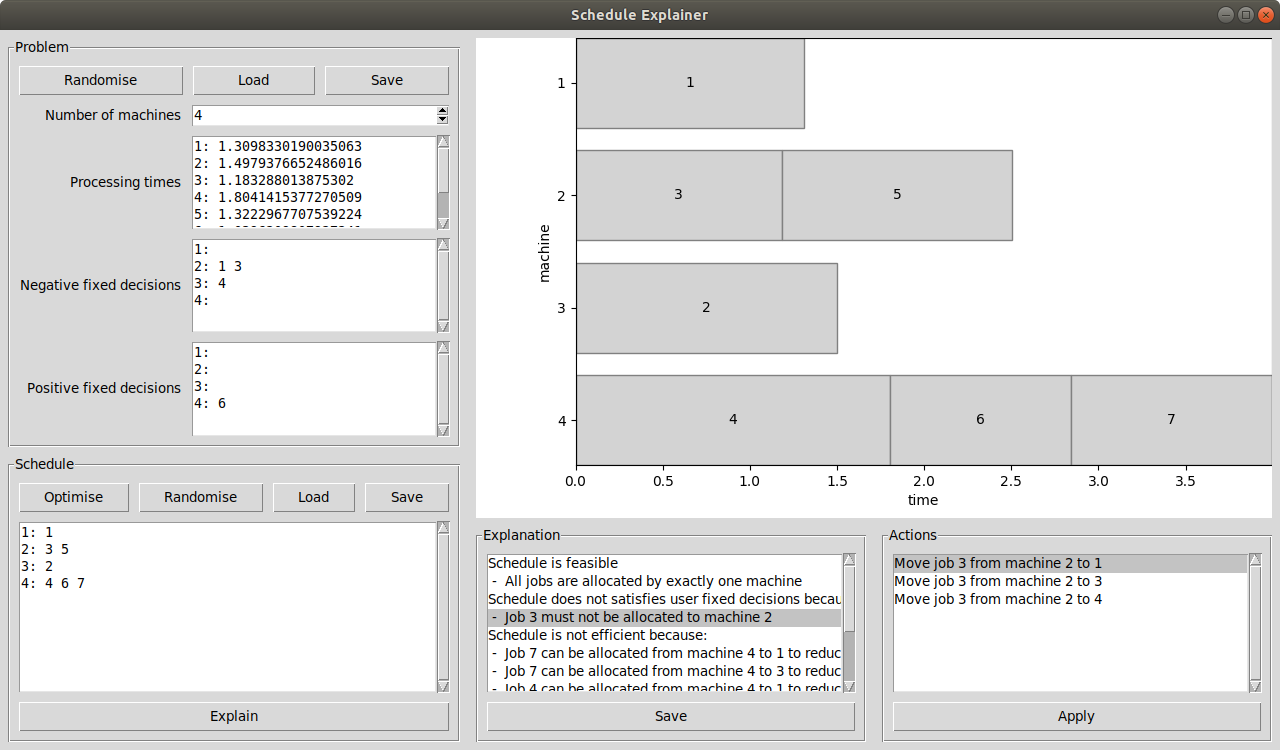
\includegraphics[width=\linewidth]{figures/tool_gui.png}
	\caption{Tool GUI}
\end{figure}

Lorem ipsum dolor sit amet, consectetur adipiscing elit. Fusce volutpat quam eu quam suscipit pharetra. Curabitur mattis nibh id metus feugiat, at blandit velit hendrerit. Quisque venenatis suscipit elit at euismod. Vestibulum ut metus vitae metus luctus tincidunt vitae eu felis. Vivamus eleifend, massa nec dignissim sagittis, eros lectus tempor neque, ac luctus magna purus ac massa. Donec fringilla arcu nec sapien varius, nec convallis justo posuere. Aenean fermentum libero erat, vitae ullamcorper diam commodo non. Nunc sodales accumsan nibh, et pellentesque sapien faucibus sed. Phasellus rhoncus dignissim orci. Aliquam maximus condimentum erat, ut porta augue euismod eu. Vestibulum ac quam ac mauris dignissim euismod vel at turpis. Curabitur nisi mauris, congue sed egestas sed, vulputate eu lorem. Donec sed semper libero. Integer diam lacus, facilisis non risus a, blandit dignissim ex. Nunc mi nulla, condimentum sit amet tellus nec, viverra gravida neque.

\subsection{Startup}

\subsection{Data Input}

\subsection{Explanations}